\documentclass[12pt,a4paper]{article}
\usepackage{minted}
\usepackage[brazil]{babel}
\usepackage[utf8]{inputenc}
\usepackage{graphicx}
\graphicspath{ {./img/} }
\usepackage{amsmath}
\usepackage{float}



\title{Relatório Práticas 2 e 3}
\author{Vitor Barbosa}
\date{\today}
\begin{document}
\maketitle
\section{Introdução}
Nestas práticas, exploramos \emph{Widgets}, propriedades e o tratamento de eventos para interfaces gráficas.
\subsection{Eventos em Qt}
Eventos em Qt usam o conceito de \emph{Sinais e Slots}.
Em suma, uma classe que deseja definir Sinais ou Slots precisa herdar de QObject, usar a macro \texttt{Q\_OBJECT} e declarar os Sinais e Slots no seu cabeçalho.
Um objeto \emph{emite} um Sinal, que pode ser conectado a uma função ou Slot.
Sinais e Slots são sempre funções de retorno \texttt{void}.

\section{A Interface Gráfica}
A IDE padrão do Qt se chama Qt Creator, e oferece um editor WYSIWYG (\emph{What You See Is What You Get}) para criação rápida de interfaces gráficas.

Tentei criar o formulário o mais próximo possível do exemplo dado pelo professor em Visual Studio e .NET. Felizmente, os Widgets disponíveis no Qt Creator são bem semelhantes.
\begin{figure}[H]
    \centering
	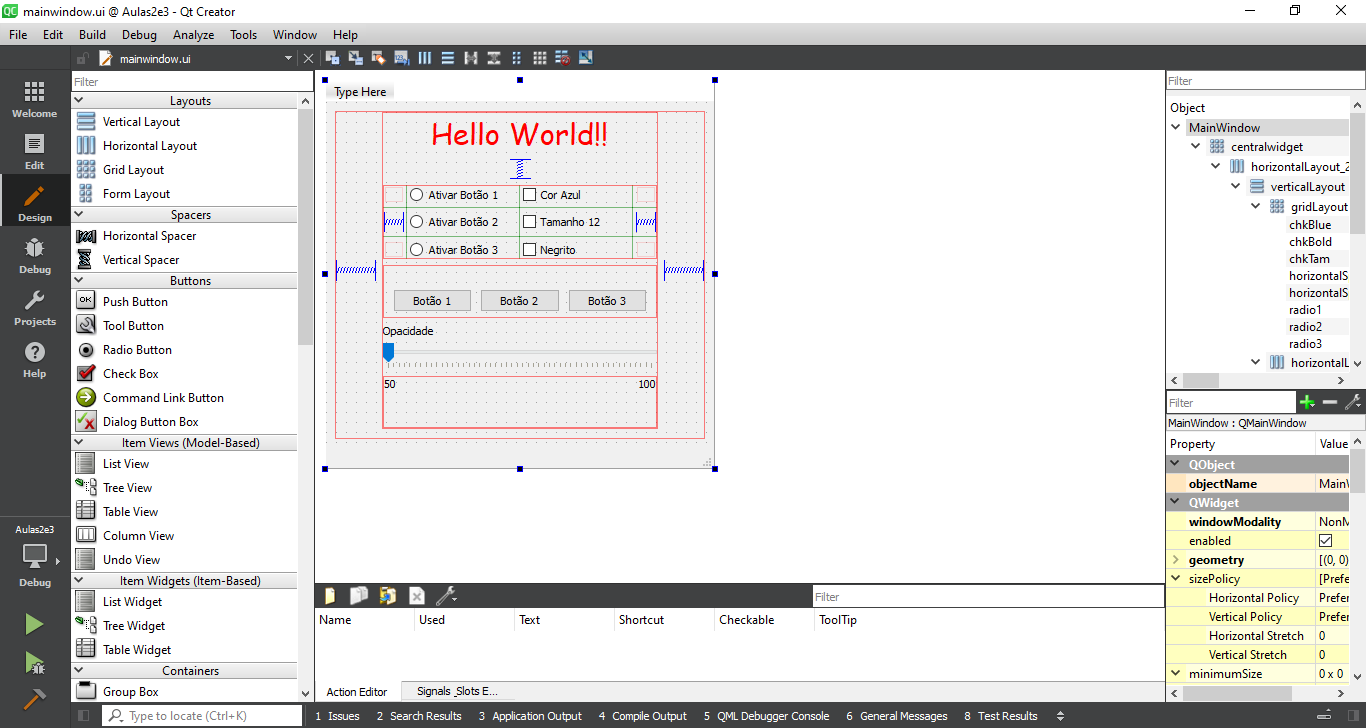
\includegraphics[width=0.95\textwidth]{wysiwyg}
\caption{Criando a janela no editor WYSIYG do Qt Creator}
\end{figure}

\section{Código}
O código possui 3 arquivos: \emph{main.cpp, mainwindow.h/cpp}.

Os arquivos \emph{mainwindow} possuem algum código gerado pela IDE, o que comumente se denomina \emph{boilerplate}.

Começamos pelo \emph{mainwindow.h}. Note que há alguns slots gerados pela IDE que começam com \texttt{void on\_ ...} 

Os slots com essa nomenclatura são conectados automaticamente aos sinais emitidos pela janela. 
\begin{minted}{cpp}
#ifndef MAINWINDOW_H
#define MAINWINDOW_H

#include <QMainWindow>
#include <QGraphicsOpacityEffect>

//Gerado pela IDE
QT_BEGIN_NAMESPACE
namespace Ui { class MainWindow; }
QT_END_NAMESPACE

class MainWindow : public QMainWindow
{
//Macro necessária para usar Sinais e Slots
Q_OBJECT

public:
MainWindow(QWidget *parent = nullptr);
~MainWindow();

private slots:
void on_slider_valueChanged(int value);

void on_chkBlue_toggled(bool checked);

void on_chkTam_toggled(bool checked);

void on_chkBold_toggled(bool checked);

private:
Ui::MainWindow *ui;
QGraphicsOpacityEffect *labelOpacity;
void hideBtns();
};
#endif // MAINWINDOW_H
\end{minted}

Arquivo \emph{mainwindow.cpp}, contém a implementação da classe.
\begin{minted}{cpp}
#include "mainwindow.h"
#include "./ui_mainwindow.h"
#include <QGraphicsOpacityEffect>

MainWindow::MainWindow(QWidget *parent)
: QMainWindow(parent)
, ui(new Ui::MainWindow)
{
ui->setupUi(this);
//Manter o alinhamento dos botões mesmo quando eles estiverem ocultos
//O comportamento padrão com layout é que eles se expandam
QSizePolicy retain = ui->btn1->sizePolicy();
retain.setRetainSizeWhenHidden(true);
ui->btn1->setSizePolicy(retain);
ui->btn2->setSizePolicy(retain);
ui->btn3->setSizePolicy(retain);

labelOpacity = new QGraphicsOpacityEffect(this);

ui->label->setGraphicsEffect(labelOpacity);
ui->label->setAutoFillBackground(true);

//Mostrando aqui uma forma alternativa para reagir a eventos simples
//Conectamos o sinal "toggled" do radioBtn a uma função lambda
//lambda c++11: [ "="( captura por valor) ou "&"(cap. ref.)]
//(opcional, parametros){corpo} -> int (opcion. valor de retorno)
QObject::connect(ui->radio1,&QRadioButton::toggled,ui->btn1,[=]{
	hideBtns();ui->btn1->setHidden(!ui->radio1->isChecked());});
QObject::connect(ui->radio2,&QRadioButton::toggled,ui->btn2,[=]{
	hideBtns();ui->btn2->setHidden(!ui->radio2->isChecked());});
QObject::connect(ui->radio3,&QRadioButton::toggled,ui->btn3,[=]{
	hideBtns();ui->btn3->setHidden(!ui->radio3->isChecked());});
}

MainWindow::~MainWindow()
{
delete ui;
}

void MainWindow::hideBtns(){
ui->btn1->setHidden(true);
ui->btn2->setHidden(true);
ui->btn3->setHidden(true);
}

void MainWindow::on_slider_valueChanged(int value)
{
labelOpacity->setOpacity(value/100.0);

}

void MainWindow::on_chkBlue_toggled(bool checked)
{
ui->label->setStyleSheet((checked?"color:blue":"color:red"));
}

void MainWindow::on_chkTam_toggled(bool checked)
{
//Copiamos a fonte atual e a reaplicamos com tamanho mudado
QFont font = ui->label->font();
font.setPointSize(checked?12:22);
ui->label->setFont(font);
}

void MainWindow::on_chkBold_toggled(bool checked)
{
QFont font = ui->label->font();
font.setBold(checked);
ui->label->setFont(font);
}
\end{minted}
Arquivo \emph{main.cpp}, gerado pela IDE, apenas instancia a janela e roda o loop de eventos principal.
\begin{minted}{cpp}
#include "mainwindow.h"
#include <QApplication>
int main(int argc, char *argv[])
{
    QApplication a(argc, argv);
    MainWindow w;
    w.show();
    return a.exec();
}
\end{minted}

\section{Resultado}
Ao rodar o programa, é aberta a janela seguinte.
\begin{figure}[H]
    \centering
    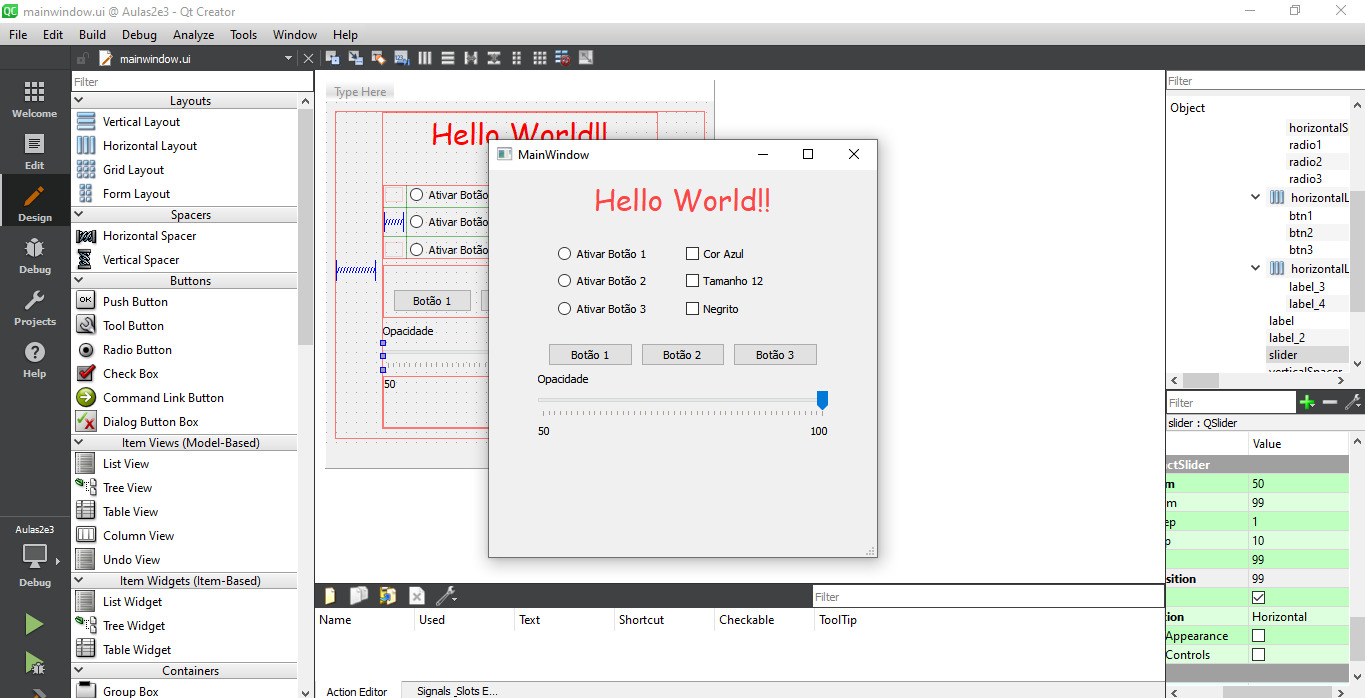
\includegraphics[width=0.95\textwidth]{demo0}
    \caption{Janela Principal}
\end{figure}
O tratamento de eventos funcionou muito bem, como pode ser visto nas duas figuras abaixo.
\begin{figure}[H]
    \centering
    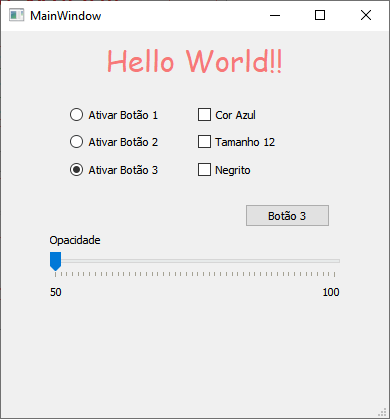
\includegraphics[width=0.5\textwidth]{demo1}
    \caption{Testando a opacidade mínima, e desativando um dos botões}
\end{figure}
\begin{figure}[H]
    \centering
    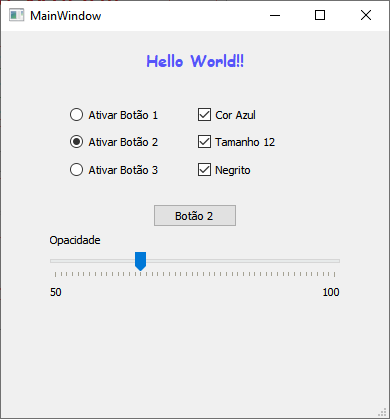
\includegraphics[width=0.5\textwidth]{demo2.png}
    \caption{Mudando opacidade, cor, tamanho, negrito e botões}
\end{figure}
\section{Referências}
https://doc.qt.io/qt-5/signalsandslots.html

\end{document}